\qns{Catenary}

In this exercise, we will show that a string suspended on both side form a convex function (c.f. Figure \ref{fig:gsi}). 

\begin{figure}[h]
\centering
\includegraphics[width=.4\textwidth]{figures/catenary.png}
\caption{Happy GSI with his representation of convex function.}
\label{fig:gsi}
\end{figure}

More formally, this exercise wants to show that a \textbf{catenary} is a convex function. 
A catenary is the curve that an idealized hanging chain or cable assumes under its own weight when supported only at its ends (Wikipedia).

Catenaries are important shapes for buildings because the internal compression forces are ideally compensated (c.f. Figure \ref{fig:bridge}).
It is also a natural form in nature as the shape minimizes free energy (c.f. Figure \ref{fig:soap}).

\begin{figure}[h]
\centering
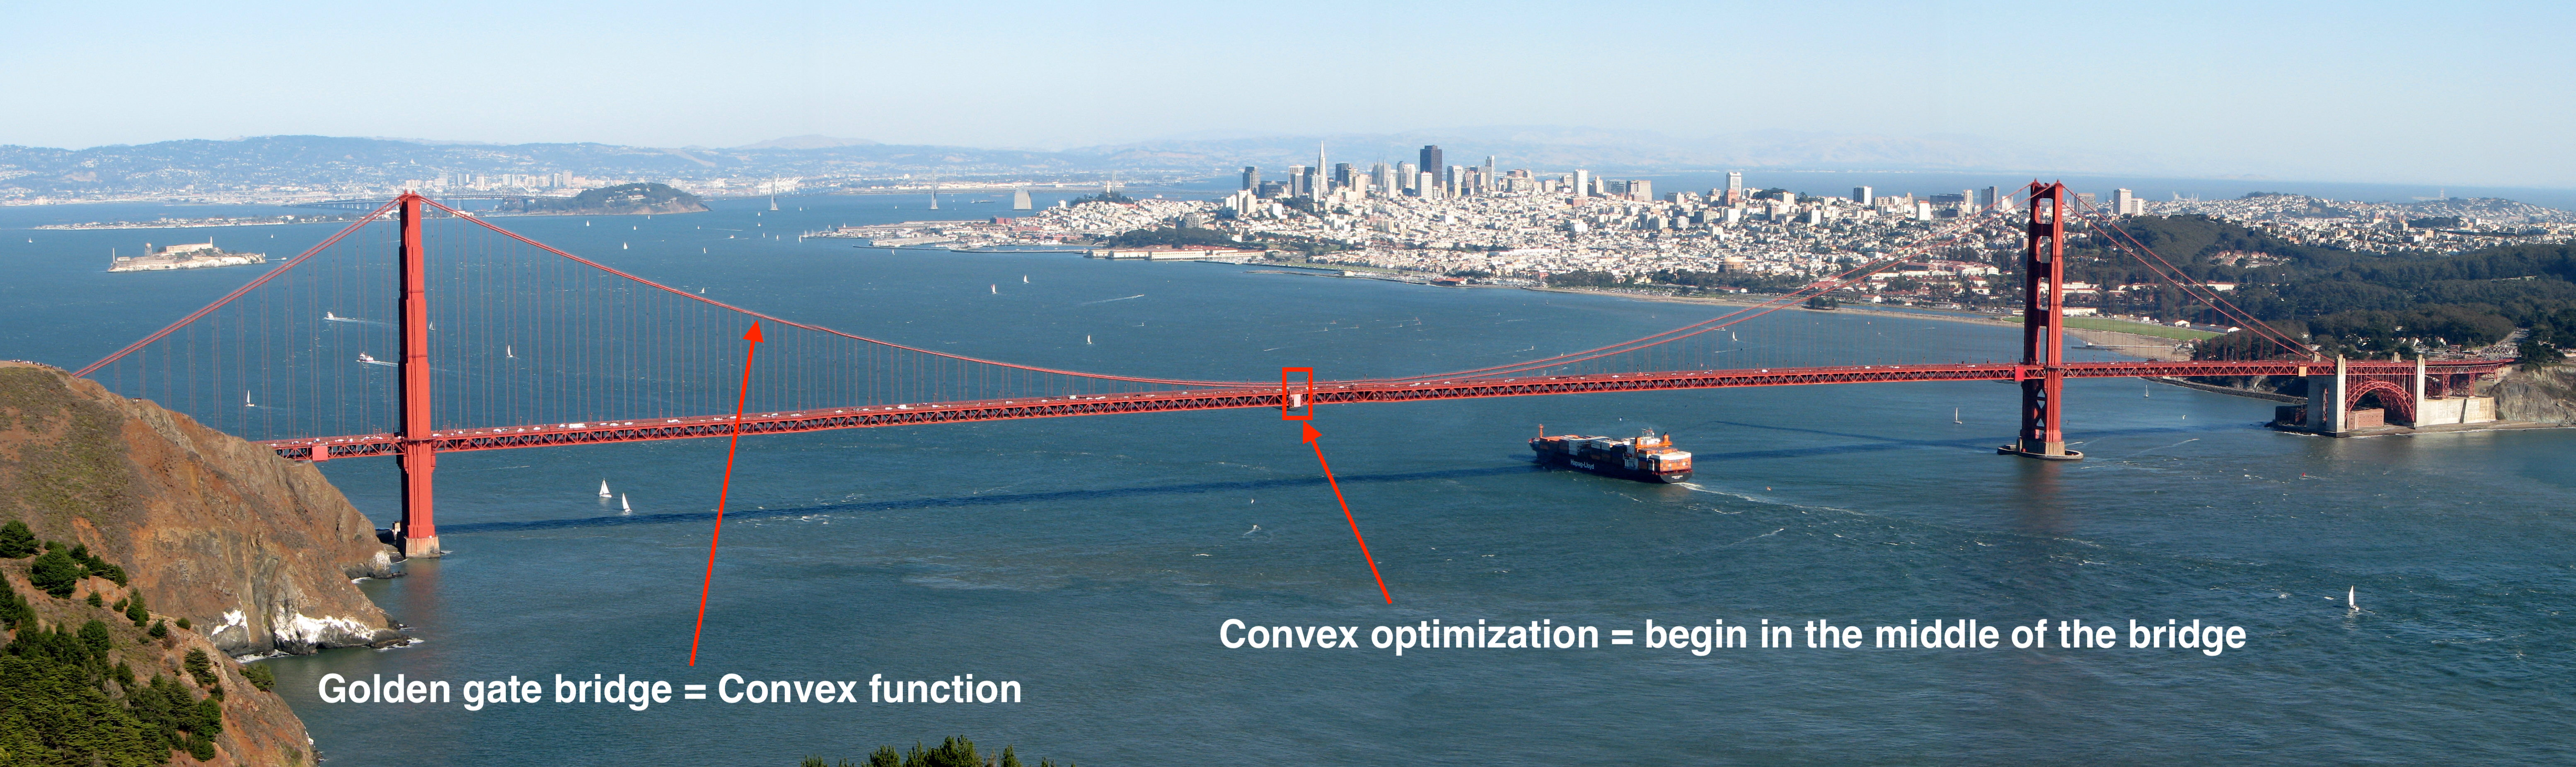
\includegraphics[width=.95\textwidth]{figures/golden_gate.jpg}
\caption{When you think about convex optimization, think about beginning in the middle of the Golden Gate Bridge!}
\label{fig:bridge}
\end{figure}

\begin{figure}[h]
\centering
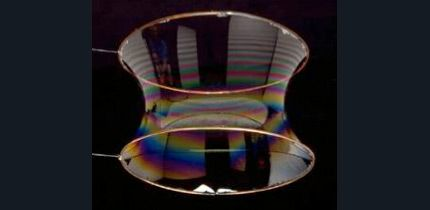
\includegraphics[width=.4\textwidth]{figures/soap.jpg}
\caption{Catenary is a shape that minimizes free energy, the vertical cut of soap film between two circles forms a catenary.}
\label{fig:soap}
\end{figure}

Let derive the equation for the catenary.
First, we need to introduce the notation (maybe the most difficult part of the exercise, see Figure \ref{fig:notations}):

\begin{figure}[h]
\centering
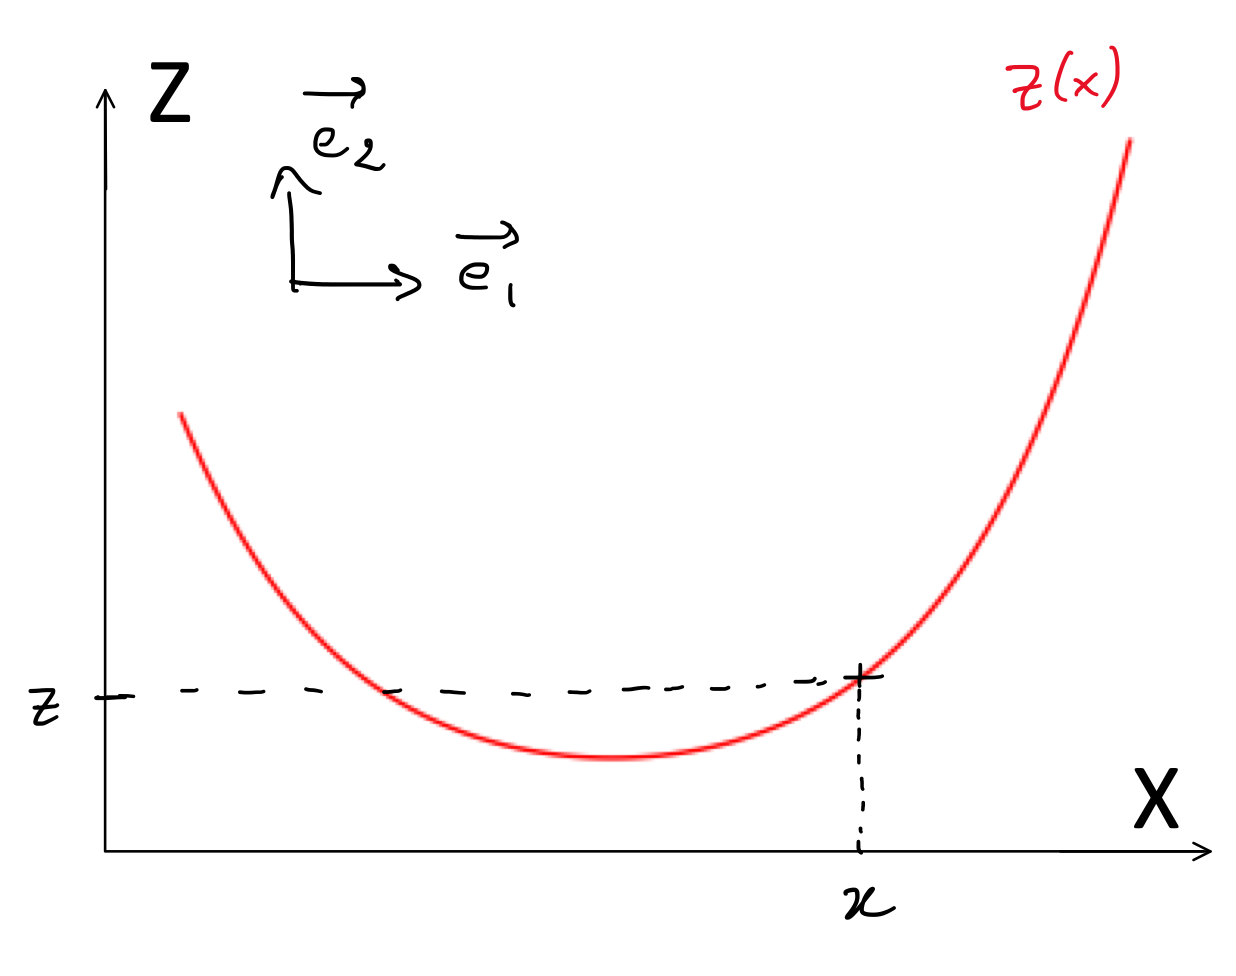
\includegraphics[width=.4\textwidth]{figures/graph.png}
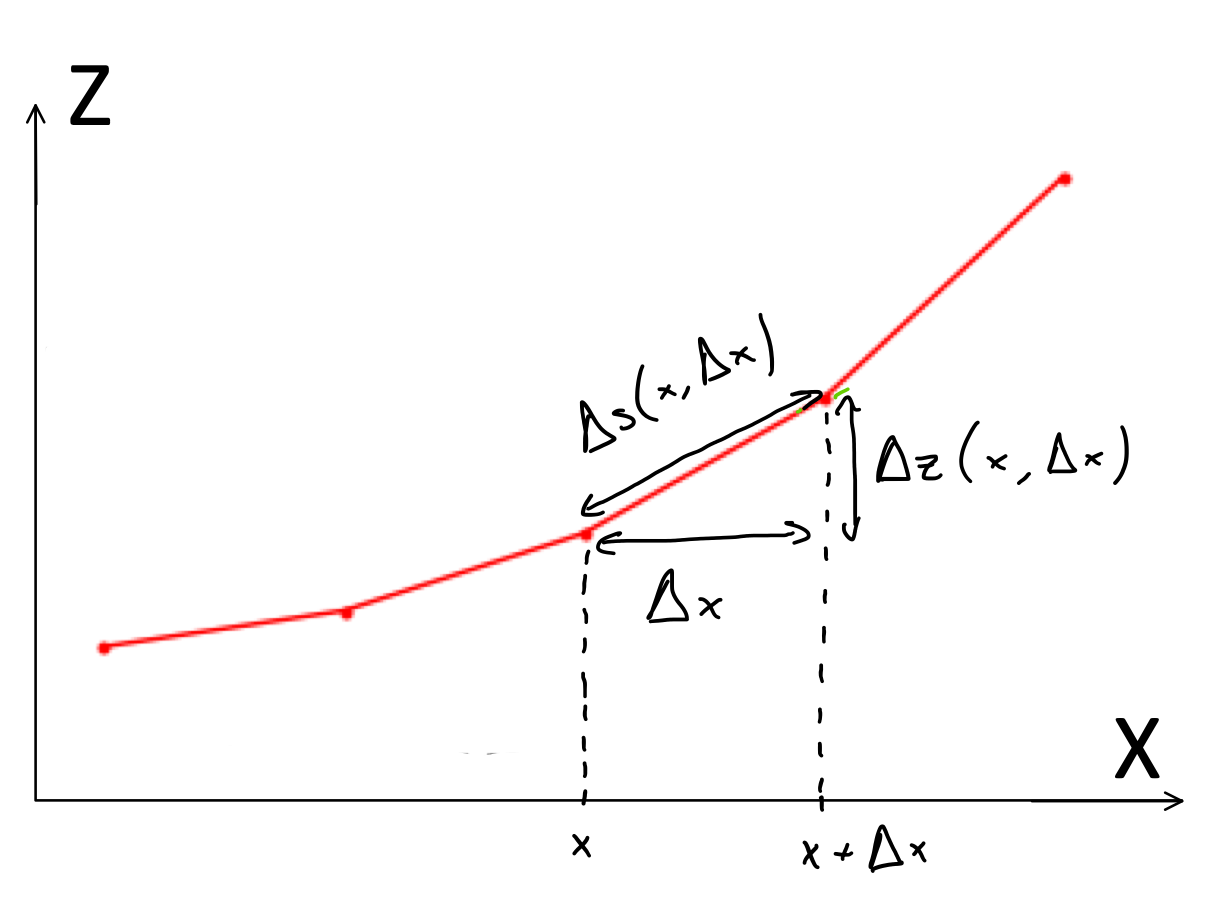
\includegraphics[width=.4\textwidth]{figures/length.png}

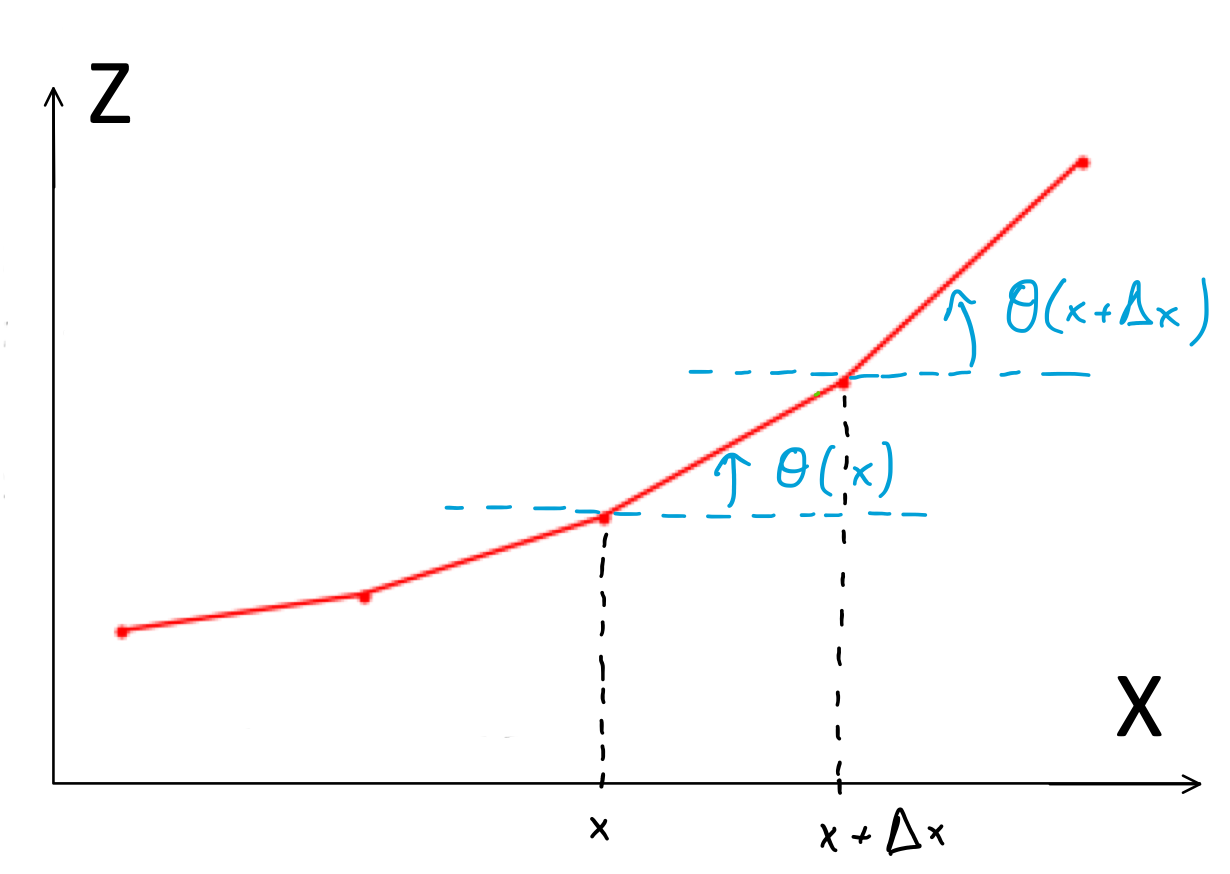
\includegraphics[width=.4\textwidth]{figures/angles.png}
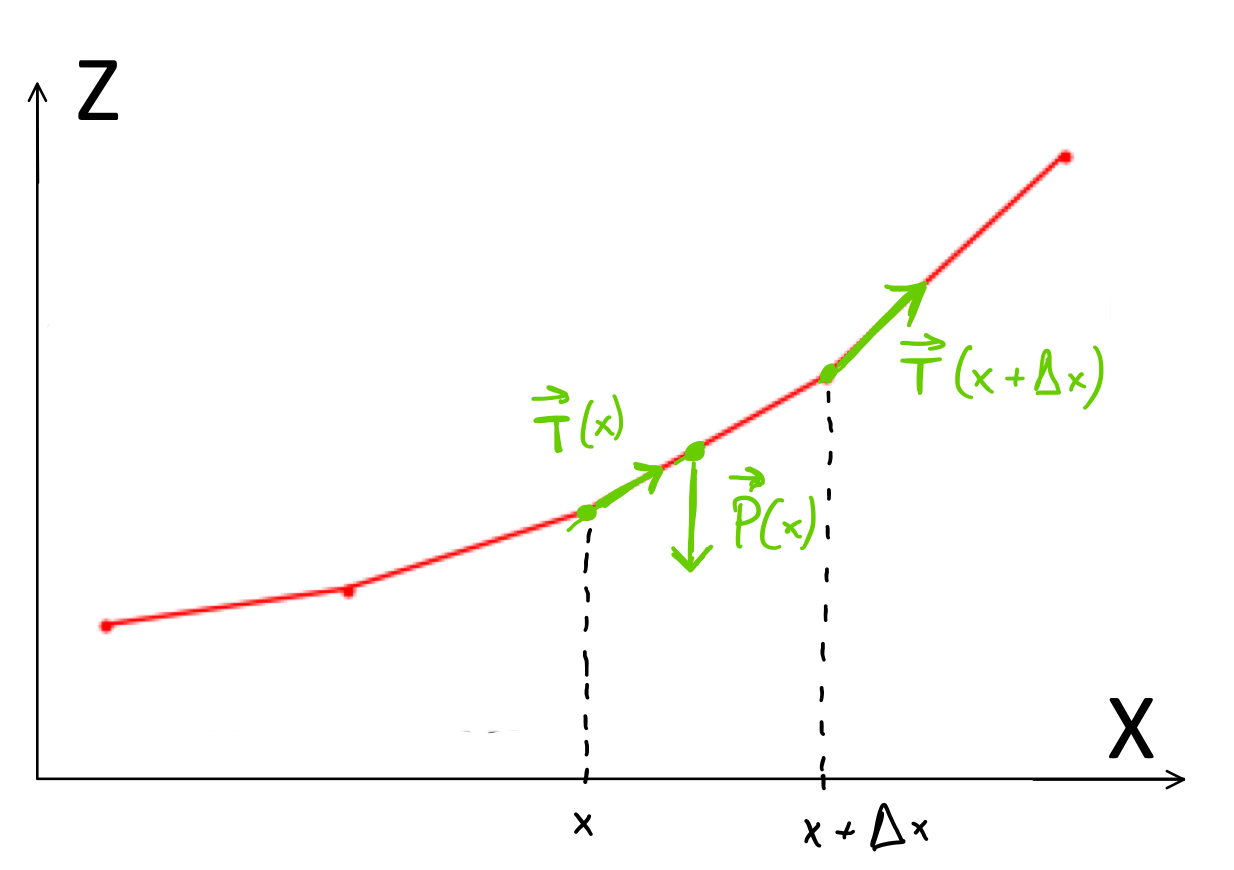
\includegraphics[width=.4\textwidth]{figures/forces.png}
\caption{Figures to help define the notation.}
\label{fig:notations}
\end{figure}

\begin{itemize}
    \item $x$ the horizontal coordinate.
    \item $z$ the vertical coordinate.
    \item $z(x)$ the equation of the catenary: we want to show that $z:x\mapsto z(x)$ is a convex function.
    \item $\Delta x$ the step for the approximation of the equation.
    \item $\Delta z(x,\Delta x) = z(x+\Delta x) - z(x)$ the vertical length at $x$ for a step size $\Delta x$.
    \item $\Delta s(x, \Delta x) = \sqrt{(\Delta x)^2 + (\Delta z(x,\Delta x))^2}$ the length of the chain between $x$ and $x+\Delta x$.
    \item $\theta(x)$ the angle between the horizontal axis and the string at $x$.
    \item $\overrightarrow{T}(x)$ the internal tension of the chain at $x$. More precisely, $\overrightarrow{T}(x)$ is the force on the segment of string to the right of $x$ due to the segment to the left of $x$.  We assume the string has no stiffness so $\overrightarrow{T}(x)$ is parallel to it, i.e.\ $\overrightarrow{T}(x) = T(x) \cos{\theta(x)} \overrightarrow{e_1} + T(x) \sin{\theta(x)} \overrightarrow{e_2}$.
    \item $\mu$ the linear density of the string.
    \item $g$ the acceleration of earth.
    \item $\overrightarrow{P}(x, \Delta x)$ the force of gravity. Physics gives us that $\overrightarrow{P}(x, \Delta x) = -\mu g \Delta s(x,\Delta x) \overrightarrow{e_2}$.
\end{itemize}

Since the string is static, the forces at each point must balance, i.e. $-\overrightarrow{T}(x)+\overrightarrow{T}(x+\Delta x)+ \overrightarrow{P}(x, \Delta x) = \overrightarrow{0}$.


\begin{enumerate}
    \qitem Show that the horizontal component of $\overrightarrow{T}(x)$ does not depend on $x$: show that $\exists T_0$ such that $\forall x,\ T(x)\cos{\theta (x)}=T_0$.
    
    \sol{\item $g(x_1,x_2) = \dfrac{x_1^2}{4} + \dfrac{x_2^2}{9}$


}
    \qitem Show that $-T(x)\sin{\theta (x)}+T(x+\Delta x)\sin{\theta (x+\Delta x)}=\mu g \Delta s(x,\Delta x)$.
    
    \sol{\item Show that the following inequalities hold for any vector $x \in \Real{n}$:
\[
% \|x\|_\infty \le \|x\|_1 \le n \|x\|_\infty \\
% \|x\|_2 \le \|x\|_1 \le \sqrt{n} \|x\|_2 \\
% \|x\|_\infty \le \|x\|_2 \le\sqrt{n}\|x\|_\infty \\
\frac{1}{\sqrt{n}}\|x\|_2 \leq \|x\|_\infty \leq  \|x\|_2 \leq \|x\|_1 \leq \sqrt{n} \|x\|_2 \le n\|x\|_\infty.
\]

\textit{Hint:} For $\|x\|_1\leq \sqrt{n}\|x\|_2$, how might you express $\|x\|_1$ as the dot product of two vectors? Can you then use the Cauchy-Schwarz inequality to bound this dot product?
    }
    \qitem Show that $- \tan{(\theta (x))} + \tan{(\theta (x+\Delta x))} = \frac{\mu g}{T_0} \Delta s(x,\Delta x)$.
    
    \sol{\item $g(x) = \sin(x_1^2) \log (x_3 - x_2)$ where $x_i$ are scalars and $x_3 - x_2 > 0$.
    }
    \qitem Show that $-\frac{\Delta z(x, \Delta x)}{\Delta x} + \frac{\Delta z(x+\Delta x, \Delta x)}{\Delta x} = \frac{\mu g}{T_0} \Delta s(x,\Delta x)$.
    
    \sol{\item
\[
g(x) = \begin{bmatrix}
x_1^2/x_2 \\
\log(x_3) \sin(x_1/x_3)
\end{bmatrix}
\]}
    
    \qitem Show that $\frac{\partial^2 z}{\partial x^2}(x) = \lim\limits_{\Delta x = 0} \frac{\mu g}{T_0} \frac{\Delta s(x,\Delta x)}{\Delta x}$.
    
    \sol{\input{catenary_solutions/5.tex}
    }
    
    \qitem Prove that $z:x\mapsto z(x)$ is a convex function.
    
    \sol{\input{catenary_solutions/6.tex}
    }
\end{enumerate}

Now we will go a little bit further in the exercise, and find the shape of the catenary explicitly.

\begin{enumerate}
    \setcounter{enumi}{6}
    \qitem Show that $\frac{\Delta s(x,\Delta x)}{\Delta x} = \sqrt{1+\left(\frac{\Delta z (x, \Delta x)}{\Delta x}\right)^2}$
    
    \sol{\input{catenary_solutions/7.tex}}
    \qitem As a first approximation, imagine that $\frac{\Delta z (x, \Delta x)}{\Delta x} \sim 0$. Show that $z(x) = ax^2+bx+c$. State the value of a.
    
    \sol{\input{catenary_solutions/8.tex}}
    \qitem Now, show that  $\frac{\partial^2 z}{\partial x^2}(x) = 
    \frac{\mu g}{T_0} \sqrt{1+\left(\frac{\partial z}{\partial x}(x)\right)^2}$.
    
    \sol{\input{catenary_solutions/9.tex}}
    
    \qitem Show that $z(x) = d\cdot \cosh{(\frac{x}{d})}$ is a solution. State the value of $d$. Compare it to the value of $a$ obtained in question (h).
    
    \sol{\input{catenary_solutions/10.tex}
    }
\end{enumerate}

\underline{Remark:} Notice that the curves of $z(x)=\frac{x^2}{2}$ and $z(x)=\cosh{(x)}-1$ are very similar around $x=0$. Indeed, $\cosh{(x)}-1 - \frac{x^2}{2} = O(x^4)$.

\underline{Remark:} Also notice that we have not shown that the solution is unique (even if this is the case).

To go further, feel free to read:
\begin{itemize}
    \item \href{https://en.wikipedia.org/wiki/Catenary}{The Wikipedia page of catenary}
    \item \href{https://www.math24.net/equation-catenary/}{The derivation of the equation of catenary on Math24.net}
\end{itemize}
